% Lecture 22

\lecture[]{2022-01-12}

Claim 5. Given a pair $(K,L)$, the theorem holds for $(L\cup\sk^m K,L)$ for all $m\ge-1$.

\begin{claimproof}
We argue by induction on $m$. If $m=-1$, $\sk^\inv K=\emptyset$, so there is nothing to show. Suppose that $m\ge0$. We set $N=K^\text{nd}_m\sm L^\text{nd}_m$. Then by proposition \ref{proposition:cw-structure-on-realization-preparation} the following is a pushout of simplicial sets:
\[
\begin{tikzcd}
\coprod_N\de\Delta^m \ar[d] \ar[r] & \coprod_N\Delta^m \ar[d]\\
L\cup\sk^{m-1}K \ar[r] & L\cup\sk^mK
\end{tikzcd}
\]
Since the theorem is true for $(\Delta^m,\de\Delta^m)$ by Claim 3, it is also true for $(\amalg_N\Delta^m,\amalg_N\de\Delta^m)$ by claim 4, then also for $(L\cup\sk^m K,L\cup\sk^{m-1}K)$ by Claim 1. Since the theorem holds for the pair $(L\cup\sk^{m-1}K,L)$ by induction, Claim 2 shows that it holds for $(L\cup\sk^mK,L)$.
\end{claimproof}

Claim 6. The theorem is true for any $(K,L)$.

\begin{claimproof}
Fix a dimension $n$. Then all simplices in $K\sm(L\cup\sk^{n+1}K)$ and all cells in $|K|\sm|L\cup\sk^{n+1}K|$ have dimension at least $n+2$, so the inclusion $L\cup\sk^{n+1}K\to K$ induces isomorphisms
\[H_n(L\cup\sk^{n+1} K,L;A)\xto{\cong}H_n(K,L;A),\] \[H_n(|L\cup\sk^{n+1} K|,|L|;A)\xto{\cong}H_n(|K|,|L|;A).\]
The theorem holds for the pair $(L\cup\sk^{n+1}K,L)$ by claim 5, hence by naturality of the $\eta$-maps:
\[
\begin{tikzcd}
H_n(L\cup\sk^{n+1}K,L;A) \ar[d,"\cong"'] \ar[r,"\cong"] & H_n(|L\cup\sk^{n+1}K|,|L|;A) \ar[d,"\cong"]\\
H_n(K,L;A) \ar[r] & H_n(|K|,|L|;A)
\end{tikzcd}
\]
it holds for $(K,L)$.
\end{claimproof}\qed

\begin{corollary}\label{corollary:adjunction-counit-is-a-weak-equivalence}
For every space $Z$, the adjunction counit $\epsilon_Z:|\S(Z)|\to Z$ induces isomorphisms of all singular homology groups.
\end{corollary}

\begin{proof}
The composite
\[\S(Z)\xto{\eta_{\S(Z)}}\S|\S(Z)|\xto{\S(\epsilon_Z)}\S(Z)\]
is the identity, hence so is the composite
\[H_*(Z;A)\xto{H_*(\eta_{\S(Z)})}H_*(|\S(Z)|;A)\xto{H_*(\epsilon_Z)}H_*(Z;A).\]
The first map is an isomorphism by theorem \ref{theorem:simplicial-and-singular-homology} applied to $\S(Z)$, hence the map $H_*(\epsilon_Z)$ is an isomorphism.
\end{proof}

\subsection{The Counit is a Weak Equivalence}

The next claim is that the counit $\epsilon_z:|\S(Z)|\to Z$ is a weak equivalence.

\begin{proposition}\label{proposition:simply-connected-realization}
Let $X$ be a non-empty simplicial set such that:\rightnote{$X_1$ is a complete graph and
\[
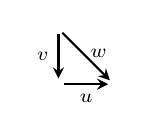
\begin{tikzpicture}[x=2em, y=2em, baseline=0.2em]
\begin{scope}[thick, -stealth, shorten >= 0.2em, shorten <= 0.2em]
\draw (0,1)--(0,0);
\draw (0,0)--(1,0);
\draw (0,1)--(1,0);
\end{scope}
\filldraw
(0,.5) node[anchor=east] {\scriptsize$v$}
(.5,0) node[anchor=north] {\scriptsize$u$}
(.4,.3) node[anchor=south west] {\scriptsize$w$};
\end{tikzpicture}
\Rightarrow\, \exists
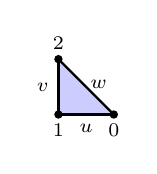
\begin{tikzpicture}[x=2em, y=2em, baseline=0.2em]
\filldraw[blue!20] (0,0)--(1,0)--(0,1);
\begin{scope}[thick]
\draw (0,1)--(0,0);
\draw (0,0)--(1,0);
\draw (0,1)--(1,0);
\end{scope}
\filldraw
(0,.5) node[anchor=east] {\scriptsize$v$}
(.5,0) node[anchor=north] {\scriptsize$u$}
(.4,.3) node[anchor=south west] {\scriptsize$w$}
(0,0) circle (1.3pt) node[anchor=north]{\scriptsize1}
(1,0) circle (1.3pt) node[anchor=north]{\scriptsize0}
(0,1) circle (1.3pt) node[anchor=south]{\scriptsize2};
\end{tikzpicture}
\]
}
\begin{itemize}[label={-}]
    \item for all $x,y\in X_0$ there is $w\in X_1$ with $d_1^*(w)=x$ and $d_0^*(w)=y$,
    \item for all $1$-simplices $u,v,w\in X_1$ such that
    \[d_0^*(u)=d_1^*(v),\ d_0^*(v)=d_0^*(w),\ d_1^*(u)=d_1^*(w),\]
    there is a $z\in X_2$ with
    \[d_0^*(z)=v,\ d_1^*(z)=w,\ d_2^*(z)=u.\]
\end{itemize}
Then $|X|$ is simply connected.
\end{proposition}

\begin{remark}
This is a special case of a more general statement. Suppose for all $0\le k\le n$ and all morphisms $\alpha:\de\Delta^k\to X$ there is a morphism $\beta:\Delta^k\to X$ that extends $\alpha$. Then $|X|$ is $(n-1)$-connected.
\end{remark}

\begin{proof}
Choose a vertex $x\in X_0$ (we will also denote with $x$ the corresponding $0$-cell in $|X|$). For each $y\in X_0\sm\cb{x}$ choose a $1$-simplex $s(y)$ from $x$ to $y$, i.e. $d_0^*(s(y))=y$ and $d_1^*(s(y))=x$. Let $T\subset X$ be the simplicial subset generated by all the $s(y)$'s and $x$. We have
\[\sk^0 X\subset T\subset\sk^{1} X\subset X.\]
Then $|T|$ is a $1$-dimensional CW-complex with $X_0$ as its set of $0$-cells and each $0$-cell is connected to $x$ by a unique $1$-cell. In particular $|T|$ is contractible. Since the inclusion $|T|\into|X|$ has the HEP ($|T|$ being a subcomplex), $|\pi|:|X|\to|X/T|$\rightnote{Secretly we are using that geometric realization commutes with colimits, hence $|X|/|T|\cong|X/T|$.} is a homotopy equivalence. Hence it suffices to show that $|X/T|$ is simply connected.

Observe first that since $T_0=X_0$, the simplicial set $X/T$ has a unique vertex $t$, so its realization is path-connected. We have
\[\sk^1(X/T)=(\sk^1 X)/T\]
and this has a unique vertex. So $|\sk^1(X/T)|$ is a $1$-dimensional CW-complex with only one $0$-cell, i.e. a wedge of circles indexed by $(\sk^1(X/T))^\text{nd}=X_1\sm T_1$. By covering space theory or Van Kampen theorem, $\pi_1(|\sk^1 X/T|,x)$ is a free group, generated by the homotopy classes of the loops:
\begin{align*}
v^\flat:[0,1]&\to|\sk^1 X/T|\\
s\ \ \,&\mapsto[v,(s,1-s)]
\end{align*}
for all $v\in X_1\sm T_1$. By cellular approximation, the map
\[\incl_*:\pi_1(|\sk^1 X/T|,x)\to\pi_1(|X/T|,x)\]
is surjective. We will end the proof by showing that all generators of $\pi_1(|\sk^1 X/T|,x)$ map to zero.

The second hypothesis provides a $2$-simplex $z\in X_2$ such that
\[d_0^*(z)=v,\ d_1^*(z)=s(d_0^*(v)),\ d_2^*(z)=s(d_1^*(z)).\]
Then the following composite:
\[
[0,1]\times[0,1]\to\sx{2}\xto{t\mapsto[z,t]}|X|\xto{|\pi|}|X/T|
\]
where the first map is $(s,t)\mapsto(t,(1-t)(1-s),(1-t)s)$, is a homotopy, relative endpoints, from $v^\flat$ to the constant loop at $x$.\alvaropls
\end{proof}

\begin{corollary}\label{corollary:simply-connected-realization-of-singular-complex}
Let $Z$ be a simply connected space.
\begin{numerate}
\item The singular complex $\S(X)$ satisfies the hypotheses of theorem \ref{proposition:simply-connected-realization}.
\item The space $|\S(X)|$ is simply connected.
\end{numerate}
\end{corollary}

\begin{proof}
We just need to prove (1), then (2) simply follows by
theorem \ref{proposition:simply-connected-realization}.\todo{Is (1) interesting on its own or is the theorem just weirdly formulated?} Let $x,y\in\S(Z)_0$ be any vertices, i.e. maps $\sx{0}\to Z$. Since $Z$ is path-connected, we can choose a path from $x$ to $y$, which we parametrize by $w:\sx{1}\to Z$ with $w(1,0)=x(1)$, $w(0,1)=y(1)$. Then $w\in\S(Z)_1$ with
\[d_1^*(w)(1)=w(d_*^1(1))=w(1,0)=x(1)\iff d_1^*(w)=x\]
and similarly $d_0^*(w)=y$.

Now we consider $u,v,w\in\S(Z)_1$, i.e. continuous maps $u,v,w:\sx{1}\to Z$. Then
\begin{align*}
    d_0^*(u)=d_1^*(v) &\iff u(0,1)=v(1,0),\\
    d_0^*(v)=d_1^*(w) &\iff v(0,1)=w(1,0),\\
    d_1^*(u)=d_1^*(w) &\iff u(1,0)=w(1,0).\\
\end{align*}
We can define a continuous (!) map $\langle u,v,w\rangle:\de\sx{2}\to Z$ by:
\[\langle u,v,w\rangle(t_0,t_1,t_2)=\begin{cases}
v(t_1,t_2) & \text{if }t_0=0,\\
w(t_0,t_2) & \text{if }t_1=0,\\
u(t_0,t_1) & \text{if }t_2=0.
\end{cases}\]
Since $Z$ is simply-connected, there is a continuous extension $z:\sx{2}\to Z$ of $\langle u,v,w\rangle$. Then we have found $z\in\S(Z)_2$ is such that $d_0^*(z)=v$, $d_1^*(z)=w$ and $d_2^*(z)=u$.
\end{proof}

\begin{theorem}\label{theorem:adjunction-counit-is-a-weak-equivalence}
For every topological space $Z$, the continuous map $\epsilon_z:|\S(Z)|\to Z$ is a weak homotopy equivalence.
\end{theorem}

\begin{proof}
Case 1. $Z$ is simply-connected and admits a CW-structure. Then by corollary \ref{corollary:adjunction-counit-is-a-weak-equivalence} and corollary \ref{corollary:simply-connected-realization-of-singular-complex}, $\epsilon_z$ is a homology isomorphism between simply-connected CW-complexes, hence a homotopy equivalence (by theorem \ref{theorem:homology-whitehead}).

Case 2. $Z$ is path-connected and admits a CW-structure. CW-complexes admit universal covers (they are locally path-connected and semi-locally simply-connected); let $\til Z\xto{p}Z$ be a universal cover. Let $G$ be the group of deck transformations of $p$. For every singular simplex $f:\ns\to Z$, we know from covering space theory that the group $G$ acts freely and transitively on the set of continuous lifts $\til f:\ns\to \til Z$, since $\ns$ is simply-connected and locally path-connected. So the morphism $\S(p):\S(\til Z)\to\S(Z)$ factors through an isomorphism $\S(\til Z)/G\to\S(Z)$.

Since $G$ acts freely on $\S(\til Z)$, the induced action on $|\S(\til Z)|$ is free and properly discontinuous, as shown in AT1Sheet11.3. Since $\til Z$ is simply-connected, so is $|\S(\til Z)|$ by corollary \ref{corollary:simply-connected-realization-of-singular-complex}, so the quotient map
\[|\S(\til Z)|\to|\S(\til Z)|/G\]
is a covering map with simply connected source, hence a universal cover of $|\S(\til Z)|/G$ with $G$ as the deck transformations group. Again\rightnote{If anyone is wondering: in $\Top$ a quotient map is the coequalizer of the diagram $R\rightrightarrows X$ where $R\subset X\times X$ is the equivalence relation inducing the quotient and the maps are the projections.}, geometric realization preserves colimits and taking orbits by a group action is a colimit, so we have isomorphisms

\[|\S(\til Z)|/G\xto{\cong}|\S(\til Z)/G|\xto{\cong}|\S(Z)|.\]

To sum up: in the commutative square of spaces (given by naturality of the counit)
\[
\begin{tikzcd}
{|\S(\til Z)|} \ar[d,"{|\S(p)|}"'] \ar[r,"\epsilon_{\til Z}"] & \til Z \ar[d,"p"]\\
{|\S(Z)|} \ar[r,"\epsilon_Z"] & Z
\end{tikzcd}
\]
since\leftnote{This argument works because $\epsilon_{\til Z}$ is $G$-equivariant, which is essentially by construction.} both vertical maps are universal coverings with isomorphic deck transformation groups, the map $\epsilon_Z$ induces an isomorphism of fundamental groups for arbitrary basepoints. Moreover, the maps $|\S(p)|$ and $p$ (being covering maps) and $\epsilon_{\til Z}$ (being a weak equivalence by Case 1) all induce isomorphisms on $\pi_n$ for $n\ge2$, hence so does $\epsilon_Z$, i.e. it is a weak equivalence.

Case 3. $Z$ is any path-connected space. We choose a CW-approximation $f:Y\to Z$, i.e. a weak equivalence with $Y$ a CW-complex. Consider the commutative square:
\[
\begin{tikzcd}
{|\S(Y)|} \ar[d,"{|\S(f)|}"'] \ar[r,"\epsilon_{Y}"] & Y \ar[d,"f"]\\
{|\S(Z)|} \ar[r,"\epsilon_Z"] & Z
\end{tikzcd}
\]
By theorem \ref{theore:singular-complex-functor-is-homotopical}, $\S(f):\S(Y)\to\S(Z)$ is a homotopy equivalence of simplicial sets, so $|\S(f)|$ is a homotopy equivalence. Hence $\epsilon_Z$ is a weak equivalence.

Case 4. $Z$ is any space. We show directly that the map $\pi_0(\epsilon_Z):\pi_0(|\S(Z)|)\to\pi_0(Z)$ is bijective. We first prove surjectivity. Any point $z\in Z$ has a corresponding map $\til z:\sx{0}\to Z$ in $\S(Z)_0$, the map $1\mapsto z$. Then $[\til z,1]\in |\S(Z)|$ is a $0$-cell in the preferred CW-structure that maps to $z$ under $\epsilon_Z:|\S(Z)|\to Z$, so $\epsilon_Z$ is surjective. For injectivity, we consider elements $[f,1],[g,1]\in|\S(Z)|$ that represent two given elements of $\pi_0(|\S(Z)|)$ that are taken by $\pi_0(\epsilon_Z)$ to the same element in $\pi_0(Z)$. We have maps $f,g:\sx{0}\to Z$. Then $f(1),g(1)\in Z$ lie in the same path component of $Z$, so there is a path $h:\sx{1}\to Z$ from $f(1)$ to $g(1)$. Then $h\in\S(Z)_1$ and the corresponding characteristic map
\begin{align*}
[0,1]&\to|\S(Z)|\\
s\ \ \,&\mapsto[h,(s,1-s)]
\end{align*}
is a path from $[f,1]$ to $[g,1]$.

Now we want to show that for any basepoint $x\in|\S(Z)|$ and all $n\ge1$
\[(\epsilon_Z)_*:\pi_n(|\S(Z)|,x)\to\pi_n(Z,\epsilon_Z(x))\]
is bijective. Fix $x\in Z$ and write $Z_x$ for the path component of $x$ with the subspace topology.\rightnote{This argument is rather subtle, but the idea is straightforward.} Then we get a commutative square
\[
\begin{tikzcd}
{|\S(Z_x)|} \ar[d,"{|\S(\incl)|}"'] \ar[r,"\epsilon_{Z_x}"] & Z_x \ar[d,"\incl"]\\
{|\S(Z)|} \ar[r,"\epsilon_Z"] & Z
\end{tikzcd}
\]
Because all $\ns$ are path connected, every singular simplex $\ns\to Z$ has image in a unique path component of $Z$. So the singular complex $\S(Z)$ is the disjoint union of the singular complexes of the path components $Z_x$ of $Z$, for $[x]\in\pi_0(Z)$, where $Z_x$ is endowed with the subspace topology. Geometric realization preserves coproducts, so it takes disjoint unions of simplicial sets to topological disjoint unions of spaces. So the left vertical map is the inclusion of the path-component of $|\S(Z)|$ that contains the point $x$. Homotopy groups beyond the zeroth only depend on the path-component of the base point. So both vertical maps induce isomorphisms on $\pi_n(-,x)$ for all $n\ge1$. The upper map is a weak homotopy equivalence by Case 3, so the lower map is also a weak equivalence.
\end{proof}
